\pdfminorversion=4
\documentclass[a4paper,12pt]{article}
\usepackage [spanish]{babel} 
\usepackage[utf8]{inputenc}
\usepackage{amsmath}
\usepackage{graphicx}
\usepackage{framed}
\usepackage{url}
\usepackage[makeroom]{cancel}

\usepackage{fancyhdr}

\newcommand{\ihat}{\hat{\textbf{\i}}}
\newcommand{\jhat}{\hat{\textbf{\j}}}
\newcommand{\khat}{\hat{\textbf{k}}}
\newcommand{\vol}{\mathop{\ooalign{\hfil$V$\hfil\cr\kern0.08em--\hfil\cr}}\nolimits}

\graphicspath{{../img/}}
 
\pagestyle{fancy}
\setlength\headheight{1.5cm}
\fancyhf{}
\rhead{
\includegraphics[width=3.0cm]{logo-mec.png}}
\lhead{
\includegraphics[width=3.5cm]{logo-utfsm.png}}
\renewcommand{\footrulewidth}{0.5pt}
\rfoot{\tiny{Departamento de Ingenier\'ia Mec\'anica}}
\lfoot{\tiny{Universidad T\'ecnica Federico Santa Mar\'ia}}

\title{Clase 9 --- Espesores de capa límite.} 
\author{Christopher Cooper}
\date{}

\begin{document}
\maketitle
\begin{framed}

Objetivos:
\begin{itemize}
    \item Entender el rol del número de Reynolds en la capa límite.
    \item Analizar la fuerza sobre una placa plana.
    \item Derivar expresiones para el espesor de la capa límite.
\end{itemize}

Contenidos:
\begin{itemize}
    \item El número de Reynolds en capa límite.
    \item La relación integral de momentum en una placa plana.
    \item Placa plana sin gradiente de presión.
    \item El espesor de capa límite de von Kármán.
    \item El espesor de capa límite de Blasius.
\end{itemize}

Bibliografía:
\begin{itemize}
    \item White, F. M. (2008) Mecánica de Fluidos. McGraw-Hill. Sexta edición. Secciones 7.2-7.4
    \item Fox, R. W., Pritchard, P. J. y McDonald, A. T. (2009) Introduction to Fluid Mechanics. John Wiley \& Sons. Secciones 9.4-9.5
\end{itemize}
\end{framed}

\section*{El número de Reynolds}

En el caso del flujo sobre una placa plana que hemos estado discutiendo, la placa se puede considerar infinitamente larga.
Esto nos p[one en una disyuntiva \mbox{?`}cuál es el número de Reynolds que caracteriza al problema entonces?
Resulta que la mejor manera que analizar estos problemas es considerando un número de Reynolds variable en el espacio.
Por lo tanto, para una misma placa plana, tendremos una distribución de números de Reynolds, donde:
%
\begin{equation}\label{eq:Re_capa}
Re_x = \frac{U_\infty x}{\nu}.
\end{equation}

Una implicancia interesante es que si analizamos en una longitud suficientemente larga, siempre vamos a llegar a número de Reynolds suficientemente altos como para empezar a ver turbulencia.
De hecho, como lo muestra la Figura \ref{fig:capa_limite_Re}, esto se ve en la práctica. 
La capa límite sobre una placa plana es siempre laminar inicialmente, y eventualmente se torna turbulenta, agua abajo.
El número de Reynolds crítico en capa límite es alrededor de $5\cdot10^{-5}$.
%
\begin{figure}[!h]
\centering
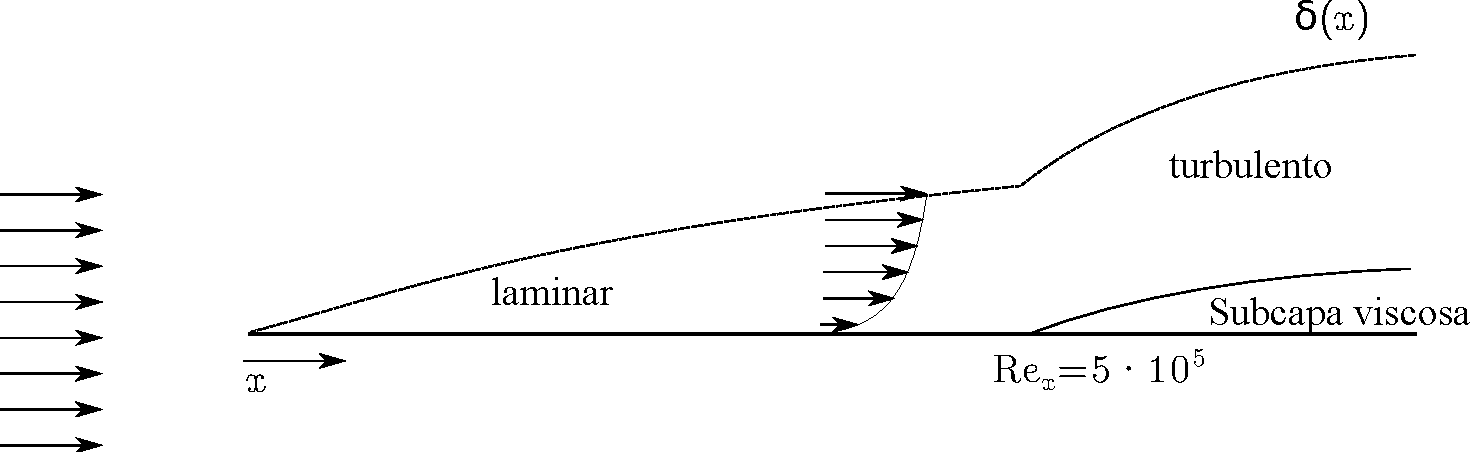
\includegraphics[width=0.8\textwidth]{clase09/capa_limite_Re.pdf}
\caption{Capa límite en función de $Re_x$.}
\label{fig:capa_limite_Re}
\end{figure}

Cuando la capa límite se torna turbulenta, aparece una pequeña zona laminar, pegada a la placa, que se conoce como subcapa viscosa.
Aparte de ser laminar, esta zona tiene importantes implicancias en el patrón del flujo dentro de la capa límite, ya que, si su espesor es mayor que la rugosidad de la placa, esta rugosidad no afecta al flujo y se puede considerar como una placa lisa. 
Como pueden imaginarse, esto tiene un importante efecto en el arrastre sobre la placa.

A continuación veremos algunas soluciones de capa límite, que dependen del número de Reynolds definido en la Ec. \eqref{eq:Re_capa}, tanto para flujo laminar, como para turbulento.

\section*{Espesor de capa límite laminar}

\subsection*{El análisis de von Kármán}
\paragraph*{La relación integral de momentum}

Quizás la forma más fácil de encontrar una expresión para el espesor de capa límite $\delta$ es a través de un análisis de cantidad de movimiento de la placa.
De hecho, la clase pasada hicimos este análisis para el caso particular en que la velocidad fuera de la capa límite $U_\infty$ sea independiente de $x$.
De no ser independiente, por Bernoulli podemos darnos cuenta que habría un gradiente de presión, y considerando que $dp/dy=0$ dentro de la capa límite, tendríamos que sumar la contribución de este $\Delta p$ a la suma de fuerzas.
Usemos la Figura \ref{fig:analisis_integral} de la semana pasada, y consideremos que el largo de .
%
\begin{figure}[!h]
\centering
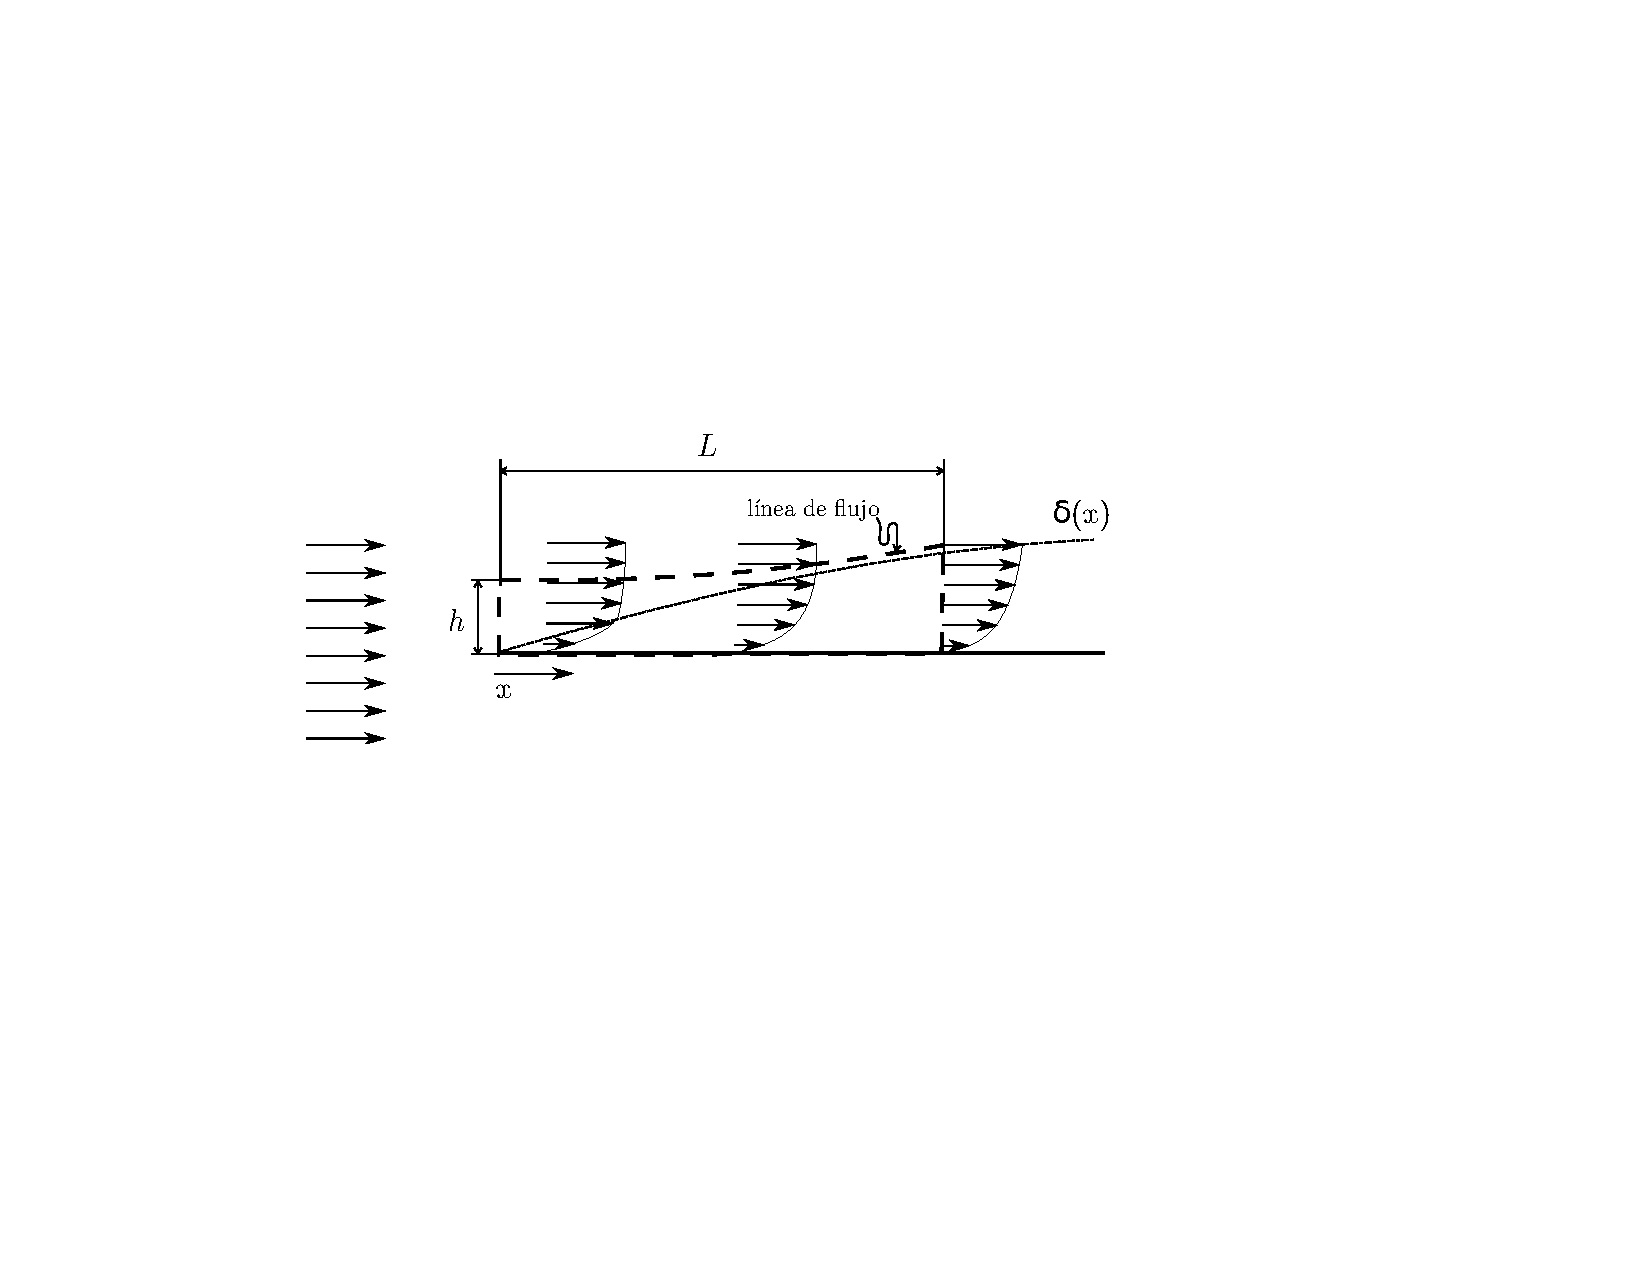
\includegraphics[width=0.8\textwidth]{clase08/analisis_integral.pdf}
\caption{Análisis integral.}
\label{fig:analisis_integral}
\end{figure}

\paragraph*{Espesor de capa límite sin gradiente de presión}

La fuerza sobre la placa $D(x)$ es el resultado de esfuerzos cortantes ($\tau_w$) a lo largo de la placa.
Matemáticamente, esto es
%
\begin{equation}
D(x) = b\int_0^x \tau_w(x)\mathrm{d}x,
\end{equation}
%
lo que implica que
%
\begin{align}
\frac{dD}{dx}=b\tau_w \text{ y, }\nonumber\\
\tau_w=\rho U_\infty^2 \frac{d\theta}{dx}.
\end{align}
%
Esta última relación se conoce como la relación integral de momentum para flujo en la capa límite sobre una placa plana.

\subsection*{Espesor de capa límite de von Kármán}

\section*{Espesor de capa límite de Blasius}



 
\end{document}
